%%%%%%%%%%%%%%%%%%%%%%%%%%%%%%%%%%%%%%%%%%%%%%%%%%%%%%%%%%%%%%%%%%%%%%%%%%%%%%%%%%%%%%%%%%%%%%%%%%%%%%%%%%%%%%%%%%%%%%%%%%%%%%%%%%%%%%%%%%%%%%%%%%%%%%%%%%%%%%%%%%%
% Written By Michael Brodskiy
% Class: Advanced Writing in the Disciplines
% Professor: L. Nardone
%%%%%%%%%%%%%%%%%%%%%%%%%%%%%%%%%%%%%%%%%%%%%%%%%%%%%%%%%%%%%%%%%%%%%%%%%%%%%%%%%%%%%%%%%%%%%%%%%%%%%%%%%%%%%%%%%%%%%%%%%%%%%%%%%%%%%%%%%%%%%%%%%%%%%%%%%%%%%%%%%%%


\documentclass[12pt]{article} 
\usepackage{alphalph}
\usepackage[utf8]{inputenc}
\usepackage[russian,english]{babel}
\usepackage[labelformat=empty]{caption}
\usepackage{titling}
\usepackage{amsmath}
\usepackage{graphicx}
\usepackage{enumitem}
\usepackage{amssymb}
\usepackage[super]{nth}
\usepackage{everysel}
\usepackage{ragged2e}
\usepackage{geometry}
\usepackage{multicol}
\usepackage{fancyhdr}
\usepackage{cancel}
\usepackage{siunitx}
\usepackage{wrapfig}
\geometry{top=1.0in,bottom=1.0in,left=1.0in,right=1.0in}
\newcommand{\subtitle}[1]{%
  \posttitle{%
    \par\end{center}
    \begin{center}\large#1\end{center}
    \vskip0.5em}%

}

\usepackage{hyperref}
\hypersetup{
colorlinks=true,
linkcolor=blue,
filecolor=magenta,      
urlcolor=blue,
citecolor=blue,
}

\urlstyle{same}
\usepackage{fancyhdr}
\pagestyle{fancy}
\lhead[\textsc{Michael Brodskiy}]{\textsc{Michael Brodskiy}}
\chead[\textsc{Education and Digital Freedom}]{\textsc{Education and Digital Freedom}}
\rhead[\textsc{\copyright 2024}]{\textsc{\copyright 2024}}
\cfoot[]{}

\usepackage{tcolorbox}


% Mathematical Operations:

% Sum: $$\sum_{n=a}^{b} f(x) $$
% Integral: $$\int_{lower}^{upper} f(x) dx$$
% Limit: $$\lim_{x\to\infty} f(x)$$

\begin{document}

\begin{center}
  
\includegraphics[width=.9\textwidth]{Images/FSFLogo.png}
\end{center}

\begin{tcolorbox}[colframe=red!65,colback=red!10]

  \underline{\textbf{The Problem}}: Though freedom-respecting (free/libre) programs predate their non-free counterparts, non-free programs have become commonplace, especially in educational environments. Although adhering to the free software philosophy would benefit all, academia should already be focused on using exclusively libre programs. Thus, for this project, I will create an opinion-editorial piece, published physically in \textit{The Huntington News}, explicating the free software movement through the scope of education, in an attempt to convince the reader to switch to more free alternatives, and possibly even begin to support the movement. This is aimed at readers involved in academia, whether student, professor, or researcher.

\end{tcolorbox}

\begin{tcolorbox}

  \begin{center}
    \underline{\textbf{Author's Note}}
  \end{center}

  \begin{flushleft}
    \hspace{.5in} Beginning the revision process, I found it best to begin by simply re-reading the entire passage. As noted by a peer, some areas appeared to be wordy and a bit too technical for someone being introduced to free software. As such, I decided it would be best to break up the article into more easily readable sections, and then focus on clarifying the ideas present within these sections. Some terms were pointed out as too technical or field specific (such as chief GNUissance), and, as such, I adjusted the piece to avoid using such terms. Most importantly, a peer mentioned that the word “clueless” generally has a negative connotation. Though I did not read it this way when I initially wrote the piece, re-reading the passage did seem to indicate that many people may be alienated by this kind of terminology. Thus, I changed “clueless” to “uninformed.” Finally, my mention of Stallman's initials, RMS, seemed to be unnecessary initially, as I continued to refer to him as Stallman, but the new revision utilizes RMS instead.\\
  \hspace{.5in} It was also pointed out that the document seems to have very limited white space, and that more spacing should be used. Though, in general, I agree that adequate use of white space is necessary, I made the decision that, since I am trying to mimic a printed article (such as a newspaper), which generally also utilize a very text-dense format, I would keep this arrangement.\\
  \hspace{.5in} As suggested, I decided to expand the problem statement a bit as well. Although the changes were minor, I thought it would be logical to add explicit statements related to where I envision this work would be published, and with what target audience. Finally, I thought it necessary to include minor edits related to overall phrasing and complexity of sentences, in order to make the piece more accessible to less technically-oriented readers.
\end{flushleft}

\end{tcolorbox}

\begin{multicols}{3}

  \section*{\small Introduction}

  WAIT! . . . see, that is exactly what your computer \textit{should} be doing . . . a computer waits to receive instructions — if it is not computing, it is waiting. But who is supplying these instructions? Is it you, or is it someone else? Your digital freedom may be at stake! With a rise in the prevalence and complexity of technology, come questions on the ethics. These questions range from privacy and tracking protection to whether companies should be able to obfuscate their code. The underlying argument of the Free Software Foundation, abbreviated FSF, essentially lies in a dichotomy: if the user does not control their system, then the system controls them. Nowadays, companies such as Microsoft, Google, Apple, and many more profit off of uninformed users by forcing them to pay, perpetually, not for the product, but for a license to be able to use said product. This immoral business model limits the users' ability to properly use the software, thereby dividing the user community and establishing the dominance of the company over the user. 

  \section*{\small The Inception of Free Software}

  Richard Stallman (generally referred to by his initials, RMS), the founder of the FSF, has been fighting for the rights of users since the early 1970s, when he graduated with a degree in physics from Harvard University, and joined the MIT Artificial Intelligence Laboratory.  RMS argues that, for a piece of software to be free (that is, free as in freedom, not price), it must follow the four freedoms: first (or the zeroth term, the way RMS numbers it), a user must be able to run the program for any purpose. Second, a user must be able to study the program and change it to their needs. Third, a user must be able to redistribute the program to help out their neighbor. Finally, fourth, a user must be able to improve the program, and release said improvements to other members of the community. 

  To provide an analogy, imagine owning a physical book. Your ability to run the code as you wish would be akin to your ability to read the book whenever you wish. The second freedom would be similar to being able to read the book, and write in the margins (whether it be notes, comments, possible changes, etc.). The third freedom would be like lending this book to your neighbor. Finally, the fourth freedom would be similar to a combination of freedoms two and three: rewriting a new revision of the book, and distributing it to other people you know.

  As such, now with codified requirements, RMS set out to create a license to benefit the community. Codified requirements were established as the GPL, or General Public License, which has since reached the third version. This is the foremost free software license (some non-FSF licenses exist), and is endorsed by the FSF. 

  \begin{wrapfigure}{l}{.6\linewidth}
  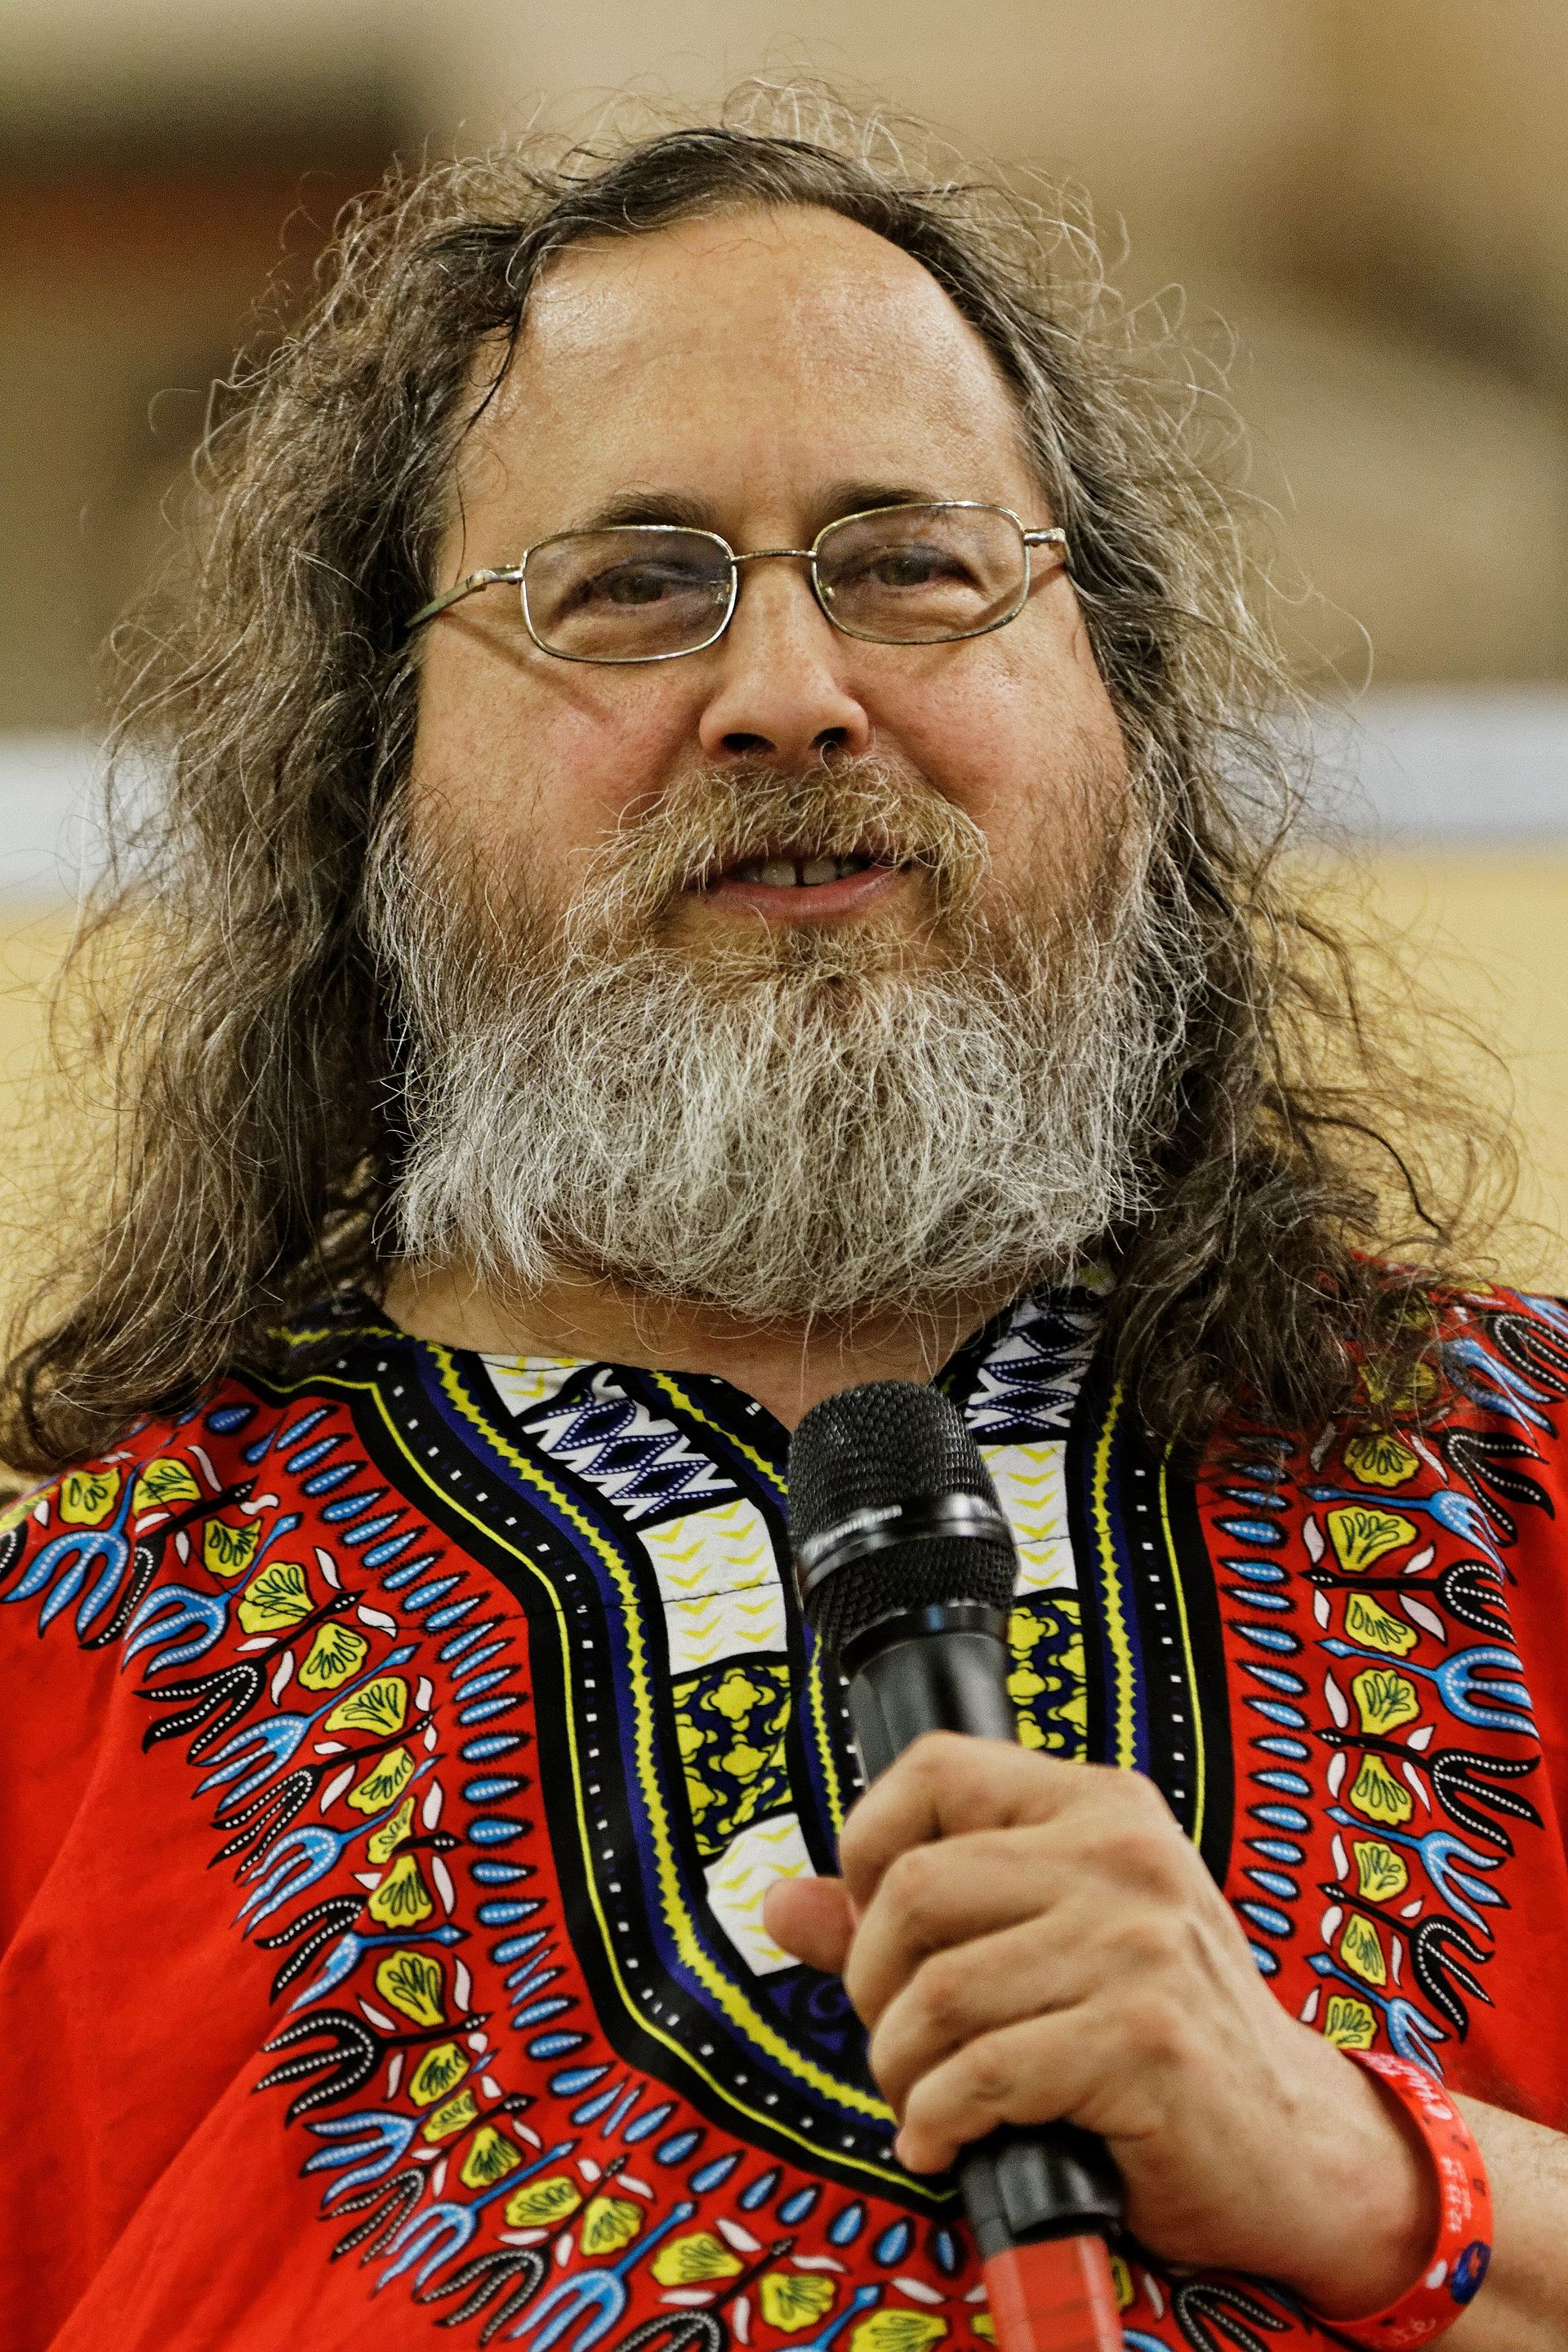
\includegraphics[width=\linewidth]{Images/Stallman.jpeg}
  \caption{\tiny Dr. Richard M. Stallman}
  \end{wrapfigure}

\section*{\small Free as in Freedom}

Of course, many questions come with the idea of “free software.” For example, it is frequently asked whether an/a individual/company may receive compensation (usually in the financial form) for creating the piece of software. Of course, this is not only allowed, but also encouraged! For example, a widely-used, real-life example lies in the Canvas Learning Management System, utilized by Northeastern University. The Canvas code itself is licensed under the AGPL (Affero GPL) license, which is commonly used for web-based software. The question about money is often asked because the main point of the FSF is misconstrued. The FSF refers to free software as relating to liberty, not price. Furthermore, the Free Software Movement concerns us, as students, in that non-free software has become ubiquitous in today's classrooms. One major example is Zoom, which has faced hundreds of privacy and rights infringement lawsuits. As is well known, due to the rise of distance learning, many schools have been faced with a transition to online learning. With this move came the need for some kind of replacement for in-person learning, and, as a result, learning establishments (as well as many companies) turned to Zoom. A great, decentralized, GNU variant is Jitsi Meet. Unlike Zoom, the user is able to host the server for meetings on their machine, without the need for an account. This means that Jitsi is private and anonymous, which makes it more efficient, as well as a safer tool for students and teachers to use. In RMS's article, entitled “\textit{Why Schools Should Exclusively Use Free Software},” RMS outlines the main reasons for schools to transfer to free systems, as well as the fiscal freedom as a byproduct of using GNU and/or free software. 

  \begin{wrapfigure}{l}{.55\linewidth}
  
\includegraphics[width=\linewidth]{Images/gnulinux.png}
  \caption{\tiny GNU/Linux Symbols}
  \end{wrapfigure}

RMS argues that schools have a social responsibility, “to teach students to be citizens of a strong, capable, independent, cooperating and free society.” As such, by using non-free software, schools are forming a dependency on the aforementioned software, thereby creating unprepared, dependent students. 

\section*{\small Misconceptions}

Often, students bring up the idea of an “educational license” that many companies, such as Microsoft, Mathworks (through MatLab), and Google give out “for free” to students. Although it may appear that this is free in price, it is ultimately the students who pay for it. These licenses are purposely made so that people are hooked to using their products, which, in the long run, will make these companies money, as students graduate and begin to pay for their licenses. Therefore, it is in the best interests of society worldwide to teach students using free software and programs. 

 \end{multicols}

 \begin{center}
   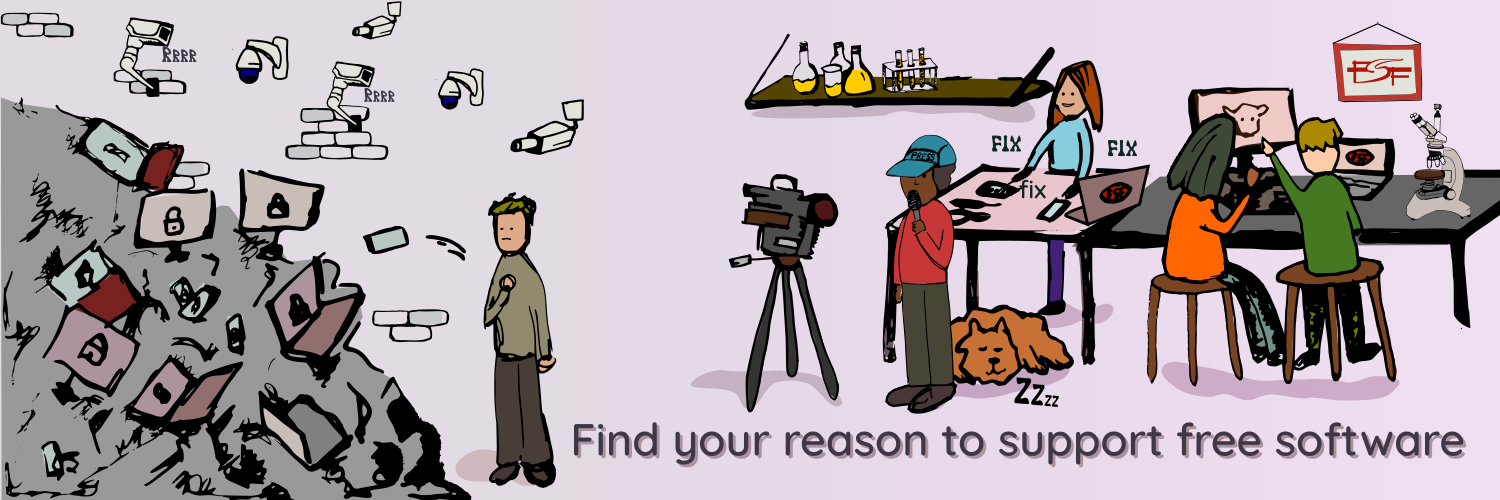
\includegraphics[width=.9\textwidth]{Images/reason.png}
 \end{center}\newpage

 \begin{center}
   \vspace{10pt}
   \underline{Interested in learning more? Check out the links below:}
 \end{center}

 \begin{center}
   \href{fsf.org}{Free Software Foundation Official Website}\\\vspace{10pt}
   \href{gnu.org}{GNU Official Website}\\\vspace{10pt}
   \href{stallman.org}{Richard Stallman's Official Website}\\\vspace{10pt}
 \end{center}

 \begin{center}
   \tiny Written and Edited by Michael Brodskiy
 \end{center}

 \begin{center}
   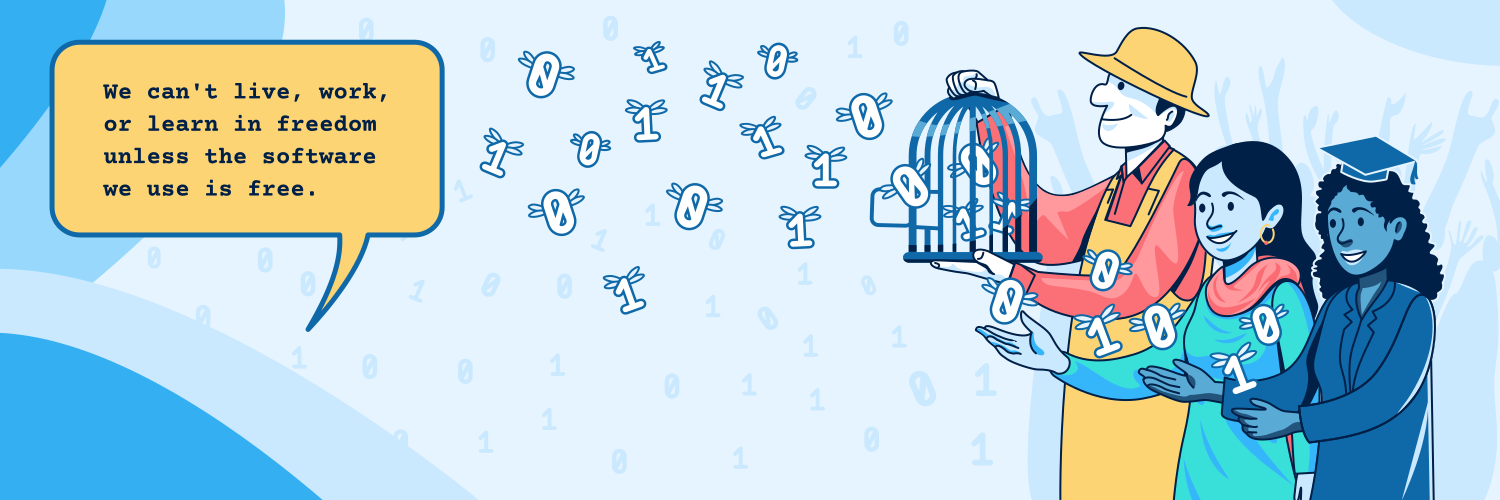
\includegraphics[width=.9\textwidth]{Images/live.png}
 \end{center}
 

\end{document}

